\chapter{Data and Methodology}
\section{Data sources and provenance}
This dissertation uses the Department for Transport (DfT) traffic count dataset as the primary data source for London. The DfT dataset provides historical traffic volumes at count points across the road network, with fields including count point id, count date, hour, all motor vehicle volume, road segment identifiers (start and end junction road names), link length, latitude, longitude, and road classification \cite{dft_counts}. The study period covers available years with full coverage for London, and records are filtered to the Greater London region. The DfT dataset is selected because it provides stable, long horizon hourly traffic volumes suitable for temporal modeling and hotspot forecasting.

The DfT counts are released on an annual cycle with hourly granularity, covering major roads and motorways. The dataset includes both automatic traffic counters and manual count points, providing comprehensive coverage of the London road network. Missingness risks include incomplete coordinates for some count points and occasional gaps in hourly records. These risks are addressed through explicit cleaning rules that drop records with missing critical fields while preserving valid observations. The dataset is used under the Open Government Licence, which permits reuse with attribution. This licensing choice is stated explicitly to ensure legal reuse and reproducibility.

Optional integration with Transport for London (TfL) disruption data is supported by the pipeline architecture but is not used in the primary analysis. The TfL Open Data API provides disruption and incident information that could enhance forecasting in future work. The current implementation focuses on DfT traffic volumes to maintain data consistency and reduce integration complexity within the MSc project scope.

\section{Data schema and dictionary}
Table~\ref{tab:dictionary} defines the core fields used for modeling and spatial outputs. Ranges are enforced during validation, and missing handling rules are applied consistently to avoid silent errors.

\begin{table}[H]
\centering
\caption{Core data dictionary used in the pipeline.}
\begin{tabular}{p{0.22\linewidth} p{0.35\linewidth} p{0.13\linewidth} p{0.12\linewidth} p{0.15\linewidth}}
\toprule
Field & Meaning & Units & Range & Missing handling \\
\midrule
count\_point\_id & DfT count site identifier & id & - & drop if missing \\
count\_date & Observation date & date & valid date & drop if missing \\
hour & Hour of day & hour & 0--23 & drop if missing \\
all\_motor\_vehicles & Volume count & vehicles & 0--20000 & cap at 99.5 pct \\
start\_junction\_road\_name & Start junction identifier & text & - & drop if missing \\
end\_junction\_road\_name & End junction identifier & text & - & drop if missing \\
link\_length\_km & Road segment length & km & 0--50 & drop if missing \\
latitude & Count point latitude & degrees & 51.0--52.0 & optional \\
longitude & Count point longitude & degrees & -0.6--0.4 & optional \\
road\_category & Road classification & category & - & keep as text \\
\bottomrule
\end{tabular}
\label{tab:dictionary}
\end{table}

\section{Pipeline, storage, and governance}
The pipeline follows a layered data lake pattern. Raw files are ingested into the bronze layer, cleaned and standardized data is stored in silver, engineered features and model artefacts are stored in gold, and light weight exports are produced for the dashboard. This layout supports auditing and partial re runs. The bronze-silver-gold pattern is chosen because it separates raw provenance from curated outputs, reducing accidental overwrites and simplifying traceability.
Figure~\ref{fig:pipeline-flow} shows the end to end flow from raw inputs to the dashboard exports.

\begin{figure}[H]
\centering
\begin{tikzpicture}[node distance=0.9cm and 0.7cm]
  \node[block] (raw) {Raw\\inputs};
  \node[block, right=of raw] (bronze) {Bronze\\raw};
  \node[block, right=of bronze] (silver) {Silver\\cleaned};
  \node[block, right=of silver] (gold) {Gold\\features + models};
  \node[block, right=of gold] (exports) {Exports\\GeoJSON + CSV};
  \node[block, right=of exports] (dash) {Dashboard};
  \draw[line] (raw) -- (bronze);
  \draw[line] (bronze) -- (silver);
  \draw[line] (silver) -- (gold);
  \draw[line] (gold) -- (exports);
  \draw[line] (exports) -- (dash);
\end{tikzpicture}
\caption{Pipeline flow from raw inputs to dashboard outputs.}
\label{fig:pipeline-flow}
\end{figure}

Storage governance follows SHU guidance. Working datasets are stored on the university networked F drive with restricted access. A backup of curated outputs is stored in AWS S3 for resilience. Access is limited to the project account, and no personal data is stored. This arrangement supports accountability and reproducibility while remaining feasible for an MSc project. The dual storage approach is used to balance institutional governance requirements with disaster recovery needs.
Figure~\ref{fig:storage-arch} illustrates the data architecture and governance controls.

\begin{figure}[H]
\centering
\begin{tikzpicture}[node distance=0.9cm and 0.9cm]
  \node[block] (shu) {SHU F drive\\primary storage};
  \node[block, right=of shu] (s3) {AWS S3\\backup};
  \node[smallblock, above=of shu] (access) {Access control\\restricted};
  \node[smallblock, below=of shu] (retention) {Retention\\policy};
  \draw[line] (shu) -- (s3);
  \draw[line] (access) -- (shu);
  \draw[line] (retention) -- (shu);
\end{tikzpicture}
\caption{Data architecture and storage governance.}
\label{fig:storage-arch}
\end{figure}

\section{Preprocessing and cleaning rules}
Preprocessing rules are explicit to prevent leakage and instability. Time alignment converts all timestamps to Europe/London time and aggregates records to hourly buckets. A combined timestamp field (ts\_hour) is constructed from count\_date and hour fields to support temporal operations. Outliers are handled by removing negative volumes and capping extreme values at the 99.5 percentile per count point. Deduplication retains the latest record when duplicate count point and hour pairs are found. Records with missing critical fields (count point id, date, hour, volume, junction names, link length) are dropped to ensure data quality. Hourly alignment is selected because the DfT data is reported at hourly resolution, which avoids artificial interpolation and maintains temporal consistency.

The cleaning stage outputs partitioned parquet files organized by year and month to support efficient querying and incremental processing. Parquet format is chosen for its columnar storage efficiency and native support in Spark. The partitioning scheme enables selective loading of time windows during model training and evaluation, reducing memory requirements and improving pipeline performance.

\section{Hotspot definition and labelling}
Hotspots are defined using a risk rate for each road segment. Predicted hourly volume is converted to a binary risk flag when it exceeds the 90th percentile of that segment's historical distribution. The hotspot rate is the proportion of hours flagged as high risk. A segment is labelled a hotspot if its hotspot rate exceeds 0.20. This threshold balances sensitivity and interpretability and avoids labeling a large fraction of the network as high risk. The percentile approach is chosen because it normalizes for segment-specific baselines and supports fair comparisons across the network.
Figure~\ref{fig:hotspot-illustration} provides a simple illustration of how hotspot labeling is applied to a map view.

The threshold is defensible because it reflects persistent risk rather than one off spikes. A 90th percentile trigger captures recurring congestion periods, while the 0.20 rate ensures the label indicates sustained exposure. This definition supports clear communication in the dashboard and aligns with policy needs for targeting interventions.

\begin{figure}[H]
\centering
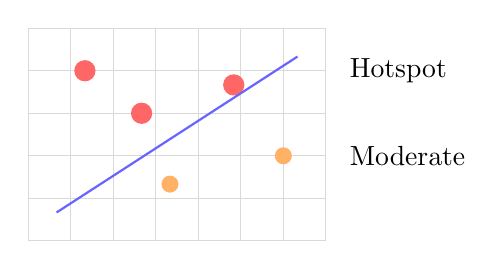
\begin{tikzpicture}[scale=0.9]
  \draw[step=0.6,gray!30,thin] (0,0) grid (4.2,3.0);
  \fill[red!60] (0.8,2.4) circle (0.15);
  \fill[red!60] (1.6,1.8) circle (0.15);
  \fill[red!60] (2.9,2.2) circle (0.15);
  \fill[orange!60] (3.6,1.2) circle (0.12);
  \fill[orange!60] (2.0,0.8) circle (0.12);
  \draw[blue!60,thick] (0.4,0.4) -- (3.8,2.6);
  \node[anchor=west] at (4.4,2.4) {Hotspot};
  \node[anchor=west] at (4.4,1.2) {Moderate};
\end{tikzpicture}
\caption{Hotspot labelling illustration for an example day.}
\label{fig:hotspot-illustration}
\end{figure}

\section{Feature engineering, modelling, validation, and ethics}
Feature engineering transforms raw traffic counts into model ready predictors. Temporal features include hour of day (0--23), day of week (1--7), month (1--12), year, and a binary weekend indicator. Lag features capture recent traffic history at 1 hour, 2 hours, and 24 hours prior to the forecast time. Rolling statistics include 24 hour mean and standard deviation computed over a trailing window. Spatial features include count point identifier and optional latitude and longitude coordinates. All lag and rolling features are computed using window functions partitioned by count point to prevent cross contamination between road segments. This feature set is deliberately compact to support interpretability and reduce overfitting risk while still capturing temporal patterns and short term inertia.

The target variable is traffic volume at a specified forecast horizon (default 1 hour ahead). This formulation supports operational forecasting where predictions are made for the next hour based on current and historical observations. The feature pipeline is implemented in Spark ML using VectorAssembler and StandardScaler to ensure consistent preprocessing across training and inference. Features are standardized to zero mean and unit variance to improve model stability and convergence.

Candidate models include Linear Regression with L2 regularization and Gradient Boosted Trees. Linear Regression provides a simple baseline that captures linear relationships between features and target. Gradient Boosted Trees handle non linear interactions and are robust to feature scaling. Random Forest is optionally available but disabled by default to reduce computational cost. Hyperparameters are selected through lightweight tuning on the first training fold and then fixed across all folds for fair comparison. Table~\ref{tab:hyperparams} summarises the final settings used in evaluation.

\begin{table}[H]
\centering
\caption{Final model parameters used in walk forward evaluation.}
\begin{tabular}{p{0.28\linewidth} p{0.64\linewidth}}
\toprule
Model & Parameters \\
\midrule
Linear Regression & regParam=0.1, elasticNetParam=0.0, maxIter=100 \\
Gradient Boosted Trees & maxIter=40, maxDepth=5, stepSize=0.1, subsamplingRate=0.7 \\
Random Forest (optional) & numTrees=40, maxDepth=8, subsamplingRate=0.7 \\
\bottomrule
\end{tabular}
\label{tab:hyperparams}
\end{table}

Walk forward validation is used to avoid leakage. Each fold trains on an expanding window and tests on the next period, with no access to future values. Metrics include MAE and RMSE for continuous prediction, and F1 and AUC for the hotspot classification derived from the forecasted volume. Calibration is reported using reliability curves for the hotspot probability threshold. Walk forward splits are preferred because random splits would leak future information into training and overstate accuracy.
Figure~\ref{fig:walkforward} defines the exact split structure used for evaluation.

\begin{figure}[H]
\centering
\begin{tikzpicture}[node distance=0.6cm and 0.6cm]
  \node[smallblock] (train1) {Train\\T1};
  \node[smallblock, right=of train1] (test1) {Test\\T2};
  \node[smallblock, right=of test1] (train2) {Train\\T1+T2};
  \node[smallblock, right=of train2] (test2) {Test\\T3};
  \node[smallblock, right=of test2] (train3) {Train\\T1+T2+T3};
  \node[smallblock, right=of train3] (test3) {Test\\T4};
  \draw[line] (train1) -- (test1);
  \draw[line] (test1) -- (train2);
  \draw[line] (train2) -- (test2);
  \draw[line] (test2) -- (train3);
  \draw[line] (train3) -- (test3);
\end{tikzpicture}
\caption{Walk forward validation with expanding training windows.}
\label{fig:walkforward}
\end{figure}

Ethics and data governance are addressed by design. All datasets are public and anonymised, with no human participants. Access to storage is restricted, and outputs are retained only for the project period before archiving or deletion in line with SHU policy. This ensures responsible use without introducing privacy risk. Restricted access is applied because governance focuses on accountability even when no personal data is present.
